\documentclass{article}

% if you need to pass options to natbib, use, e.g.:
% \PassOptionsToPackage{numbers, compress}{natbib}
% before loading nips_2016
%
% to avoid loading the natbib package, add option nonatbib:
% \usepackage[nonatbib]{nips_2016}

\usepackage[final]{nips_2016}

% to compile a camera-ready version, add the [final] option, e.g.:
% \usepackage[final]{nips_2016}


\usepackage[utf8]{inputenc} % allow utf-8 input
\usepackage[T1]{fontenc}    % use 8-bit T1 fonts
\usepackage{hyperref}       % hyperlinks
\usepackage{url}            % simple URL typesetting
\usepackage{booktabs}       % professional-quality tables
\usepackage{amsfonts}       % blackboard math symbols
\usepackage{nicefrac}       % compact symbols for 1/2, etc.
\usepackage{microtype}      % microtypograph
\usepackage{textcomp}
\usepackage{gensymb}
\usepackage{graphicx}
\usepackage{algorithm}
\usepackage[noend]{algpseudocode}

\title{Bayesian Methods in Target Motion Analysis}

% The \author macro works with any number of authors. There are two
% commands used to separate the names and addresses of multiple
% authors: \And and \AND.
%
% Using \And between authors leaves it to LaTeX to determine where to
% break the lines. Using \AND forces a line break at that point. So,
% if LaTeX puts 3 of 4 authors names on the first line, and the last
% on the second line, try using \AND instead of \And before the third
% author name.

\author{
  Joe Goldfrank\\
  Department of Management Science \& Engineering\\
  Stanford University\\
  \texttt{goldrank@stanford.edu} \\
  %% examples of more authors
  \And
  David Liedtka \\
  Department of Computer Science \\
  Stanford University\\
  \texttt{dliedtka@stanford.edu} \\
  \AND
  Greg Forbes \\
  Department of Civil \& Environmental Engineering \\
  Stanford University \\
  \texttt{gforbes@stanford.edu} \\
}

\begin{document}
% \nipsfinalcopy is no longer used

\maketitle

\begin{abstract}
  We investigate applications of nonlinear state estimation and approximate dynamic programming to target motion analysis problems for which deterministic solutions are inadequate, such as problems with low sensor accuracy or intermittent contact. We demonstrate methods for an example problem with competing objectives: maintaining target track and avoiding collisions using a generic side-looking intermittent-contact linear array sensor. We use sequential importance sampling particle filter state estimation, and Monte Carlo Tree Search and global-approximation naïve Q($\lambda$) learning solution methods. These techniques have applications .
\end{abstract}

\section{Introduction}
\par We investigate the case of tracking and search of a two-dimensional space by a mobile sensor, where the sensor is directional and has sensor axis fixed in relation to the mobile sensor's direction of motion. Pointing the sensor affects both \textit{what it is looking at} as well as \textit{where it is moving to}. The mobile sensor will be used to search for a non-cooperative mobile target and should be able to locate the target and then maintain continuous contact with (follow) the target indefinitely. Collision with the target is possible and should be avoided.
\par Many types of sensors benefit from having as large an aperture size as possible; a mobile sensor-- a sensor integrated with a vehicle-- can have a smaller overall size by having the sensor be of fixed direction, as this removes all machinery required to move the sensor relative to the vehicle. Examples include, but are not limitekeepd to, side-scanning sonar common on Unmanned Underwater Vehicles and certain search radars used on aircraft and spacecraft. Decision-makers must actively manage the relationship between vehicle positioning and sensor employment.
\par Furthermore, because of physical configuration, these sensors are often side-looking; because of drag, vehicles in fluid domains are often `long and thin.' Aperture size is maximized by using the length of the vehicle, resulting in a side-looking sensor. Due to the geometry of beamforming, these sensors' resolution is not uniform with respect to relative bearing: resolution may be excellent at 90\textdegree \, relative and mediocre at 30\textdegree \, relative to the direction of sensor motion.[1] Pointing the mobile sensor therefore affects the vehicle's motion, where it is looking, and how well it is covering those areas.
\par As Partially-Observable Markov Decision Processes (POMDPs) and Reinfrocement Learning have successfully been applied to other target tracking and collision-avoidance problems, we selected these methods for application to this use case.


\section{Related Work}
\par Work related to our analysis spans the literature of linear array beamforming, controls and algorithms for unmanned systems, Reinforcement Learning and POMDP use for target tracking of unmanned systems, and unmanned system collision avoidance.

\par Control systems and algorithms of autonomous systems is an active area of research in aeronautics, astronautics, and robotics. Sensing and control for vehicles in numerous domains has been demonstrated with methods ranging from rules-based algorithms to POMDPs and deep reinforcement learning. W. Schwarting et al.\ provide a recent survey of methods.[2]

\par The work performed by C. Eaton et al.\ provided more in-depth techniques within the literature regarding the methods and capabilities of path-planning and target tracking. This work categorizes the path planning as fixed target, moving target, and target search and surveillance, with emphasis on the advancement of the later. Recommendations have been provided to emphasize research in sensor and sensor data for decision-making so that autonomous control methods can be better enabled when following a desired target(s).[3]

\par POMDPs have more recently been implemented in target search and surveillance tasks. S. Ragi et al.\ tracks multiple targets by taking advantage of the flexibility of the POMDP structure. This work incorporates a variety of parameter features including variable-speed, aerodynamic drag, collision avoidance, and track swap, among others. The utility of this work is derived from the generality and flexibility of POMDPs, which recommends their use as a framework to incorporate other features of interest in target search and surveillance problems.[4]


\section{Methods}
\label{headings}
\subsection{Problem Structure}
\par We modeled a simplified discrete-time discrete-action target search repesenting the constraints of Section 1 in the Julia programming language. Our state space used relative polar coordinates, and was comprised of relative distance $r$ and angle $\theta$ of the target to the sensor, the target's relative course, and the sensor's speed. The target speed was modeled as fixed. The target's motion was modeled as a random walk, maintaining course with probability 0.9 and turning either l30\textdegree \,  left or 30\textdegree \, right, each with probabiltiy 0.05. The action space consisted entirely of sensor course and speed maneuvers: 0\textdegree \, (no change),  30\textdegree \,  left,  or 30\textdegree \, right course changes, and speed either equal to or twice the target's speed. All actions were available from all states.

\par The sensor was modeled as an approximation of a on-motion-axis linear array with a forward null, as shown in Figure 1.
%\begin{figure}[h]
%  \label{fig:sensor_config}
%  \centering
%  \includegraphics[width=0.75\textwidth]{TMA6.png}
%  \caption{Sensor Configuration}
%\end{figure}
\clearpage

\par Observations are based on $r$ and $\theta$ at each time step. If the target is in an observation zone and closer than distance $R$, that zone's observation will occur at the time step. If the target is in an observation zone with range between distances $R$ and $R'$, that zone’s observation occurs with probability inversely proportional to relative distance ($\frac{1}{r}$) from the sensor. If the target is not in any observation zone, no observation occurs at the time step.

\par We performed state estimation using a Sequential Importance Resampling Particle Filter implemented using the \texttt{ParticleFilters.jl} library.[7] State estimation performance was validated with test cases prior to implementing the problem solution methods.

\subsection{Reinforcement Learning}

\par We implemented several variations of the Q-learning family of algorithms described in [5] and [6]: global-approximation Q-learning, global-approximation Watkins's Q($\lambda$), global-approximation naïve Q($\lambda$), and local-approximation naïve Q($\lambda$). A variation of global-approximation naïve Q($\lambda$) demonstrated the best performance.

\par We implemented a polar-coordinate coordinate approximation scheme by extending the multilinear grid interpolation \texttt{GridInterpolations.jl} package[8] to use polar coordinates, accounting for the behavior of state variable $\theta$ by introducing a 360\textdegree \, state that is merged with the 0\textdegree \, state after interpolation.

\par We used this coordinate approximation scheme for global approximation rather than local approximation by adding the weights of each particle in the particle filter into a combined state, and then taking the variance of these weights to generate an additional synthetic state representing variance of particle distribution. This method is shown in Algorithm 1.

\begin{algorithm}[H]
    \caption{Global Approximation With Variance}
    \begin{algorithmic}[1] % The number tells where the line numbering should start
        \Function{Global Approximation}{$particles$}
          \State Initialize $\beta$
          \For{$p \in particles$}
              \State $\xi \gets \textsc{Interpolants}(p)$
              \State $\beta \gets \beta + \xi$
          \EndFor
          \State \textsc{Normalize}($\beta'$)
          \State $\nu \gets var(\beta)$
          \For{$\vec{b} \in \beta$}
              \State $b \gets \textsc{Concatenate}(b, \nu)$
          \EndFor
          \State \textbf{return} $\beta$
        \EndFunction
    \end{algorithmic}
\end{algorithm}

We included three synthetic ``variance" states in the cooridnate approximation scheme, corresponding to high, medium, and low variance, tunable with a hyperparameter. The global approximated state was then used in a naïve Q($\lambda$) algorithm until desired performance was achieved.

\subsection{Monte-Carlo Tree Search }
\par In addition to offline reinforcement-learning-based methods, we also computed an online solution, in which real-time computation determines the action taken. The problem dynamics suggested that satisficing solutions exist and optimality was not required. To this end,  we implemented a modified version of Monte Carlo Tree Search (MCTS) extended to POMDPs. Computational load is reduced by only interrogating states reachable within a finite time horizon from the current state.

\par Our MCTS implementation is largely identical to that of Algorithm 6.12 of [5], the sole difference being that instead of recycling past computation by advancing the history tree after selecting an action, we achieved best results by reinitializing the algorithm at each time step. We believe this is due to specific problem dynamics: observations correspond to wide ranges of states (for which different actions maximize reward) and individual rewards to do not unambiguously resolve target bearing.

\par The other implementation choices we made were terminating the loop over MCTS simulations after 100 iterations and using a random rollout policy. While we considered that in practice one might continue iterating until a decision must be made (which we could have achieved using a timed loop), we found the algorithm had converged by 100 iterations and continued iterations thus wasted computation--- as this algorithm would be run in real time, we are sensitive to its computational complexity. For our rollout policy, we chose random actions until we reached the specified depth.

\section{Simulations}

\par For each simulation, we chose a starting state (with a random range $r$ between 25 and 100, a random relative bearing $\theta$, a random relative course, and vehicle speed of 1) and assumed perfect knowledge of the initial state. We implemented a reward function based only on state, with a large negative reward for a collision, a small negative reward for the target range exceeding the maximum sensor range, and a small positive reward otherwise. We then iterated over 500 time steps, ending the simulation early if the sensor collided with the target.

\subsection{Reinforcement Learning}
\par For the global-approximation naïve Q($\lambda$) approach, we impemented both softmax and $\epsilon$-greedy exploration strategies, decreasing the exploration rate both over time and in response to algorithm performance (average reward over a set number of training epochs). We found that the performance was extremely sensitive to choices of discount factor $\gamma$, eligibility trace discount factor $\lambda$, learning rate $\alpha$, and to the exploration strategy, with $\alpha = 0.7$, $\gamma = \lambda = 0.9$ with $\epsilon$-greedy performing well. Results are detailed in Section 5.

\subsection{Monte-Carlo Tree Search}
\par For MCTS, we first ran experiments over up to 100 trials to tune parameters before running an experiment over 1,000 trials with our optimal set of parameters. The tunable parameters were the depth $d$, the exploration constant $c$, the discount factor$\lambda$, and the number of iterations per action chosen. We used values of $c = 20$, discount factor $\lambda = 0.95$, and 100 iterations, and experimented with depth parameters of 1, 5, 10, 25, and 100. However, as explained further in Section 5, we achieved maximum reward in all of our trials for all depths excluding depth 10. Thus, there was no need to tune the other parameters and we chose to use a depth of 1 since it required the least computation (with a depth of 1 we could run roughly 60,000 MCTS simulations per second, but only 2,500 per second with a depth of 100\footnote{Single-threaded on an 8th-generation Intel i7 x86 processor.}). Additionally, we conducted MCTS experiments without assuming perfect knowledge of the initial state (we assumed only that we knew the target was somewhere between range 25 and 100 and that our own speed was 1).

\section{Results and Discussion}
\par We measured performance by per-epoch tracking loss percentage and collision percentage over 500 time steps. A random action policy measured over 12,000 epochs resulted in 47.5\% tracking loss rate and 15.4\% collision rate.

\subsection{Reinforcement Learning}
\par As mentioned in Section 4, the global-approximation naïve Q($\lambda$) approach was very sensitive to choices in hyperparameters, and would converge on a good policy very slowly when we chose these parameters poorly. We ran the algorithm on small-time step epochs to determine better hyperparameter choices, and then ran the best-performing combination for 20,000 500-time-step training epochs. We then tested our results over 2750 training epochs, measuring a 0.95\% tracking loss rate and a 0.54\% collision rate, greatly improved performance compared to the random policy. An example policy result (representing only two of five state dimensions) is shown in Figure 2. Each color represents one of the six possible action choices.

%\begin{figure}[h]
%  \label{fig:heatmap}
%  \centering
%  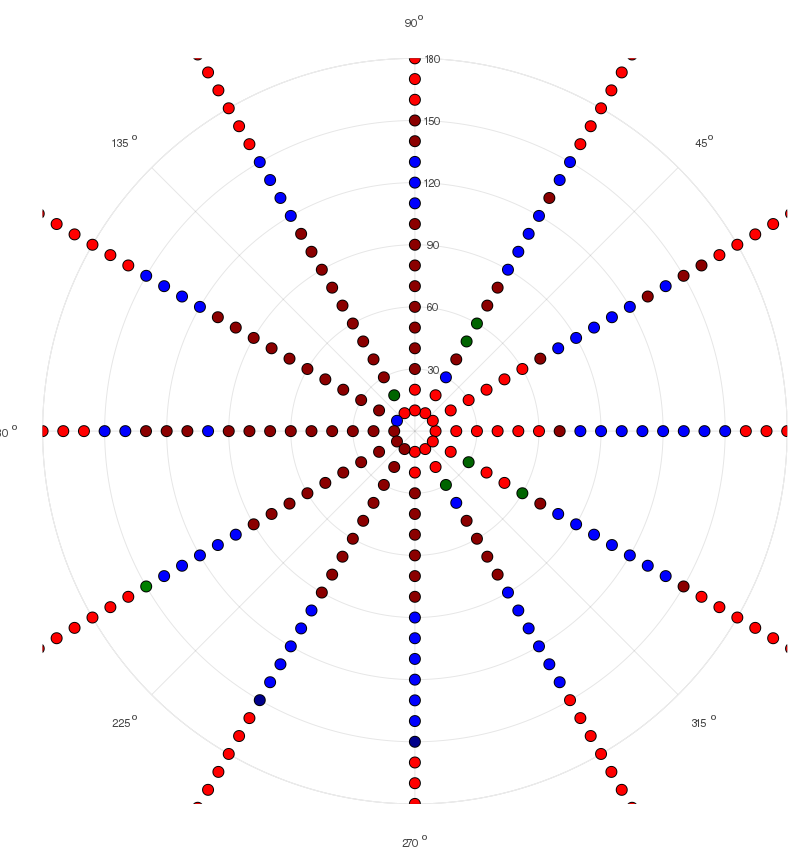
\includegraphics[width=0.75\textwidth]{heat.png}
%  \caption{Policies at Approximation Points}
%\end{figure}

\par We had previously implemented the other variations on Q-learning and Q($\lambda$), but these did not achieve good results until we added the synthetic state to account for particle filter variance. While we qualitatively recognize why accounting for degree of state uncertainty improves the algorithm's performance, we do not yet have a method for quantifying this performance improvement.\footnote{We were not able to find examples of this technique in a survey of the literature, but look forward to the teaching team's feedback regarding other implementations and methods for improvement.}

\subsection{Monte-Carlo Tree Search}
\par MTCS performed perfectly (no tracking losses or collisions) for depths of 1, 5, 25, 50, and 100 (there was a non-zero tracking loss rate for depth 10) up to 100 trials. Then, we chose the least computationally intensive depth of 1 and found that MTCS performed perfectly for each of 1,000 random trials. Additionally, we replicated the same success with MCTS over 1,000 trials when we did not assume perfect knowledge of the start state (we randomly initialized our particle filter belief state in the range of 25 to 100).

We suspect MCTS was effective using a depth of 1 due to the relatively forgiving problem structure and the effectiveness of the particle filter. The likelihood of the target changing course at any time step is low, allowing our vehicle to effectively take action to avoid negative reward states before being reached. Because the particle filter works well, the vehicle takes these preventive actions with high certainty.

While it is unclear exactly why depth 10 performed worse over 100 trials than lesser and greater search depths, we suspect that at this depth there was greater potential for generative simulations to separate from actual outcomes but there was not enough depth to allow for correction.  We likely could have remedied this problem by tuning $\lambda$, but with better solutions available there was no need to do so. We also recognize that a larger number of trials would have yielded different results for other depths.

MTCS was the best-performing of our solution approaches, and was able to continuously track the target without loss of contact or collision. Additionally, we avoided the need for discretization of states, being able to track continuous states using particle filter state estmation and randomly sampling the population of particles. Finally, the assumptions required of the initial state were minimal, and MCTS requires no prior training.

The drawback of MCTS is that, as an online method, it requires real-time computation and cannot execute deterministically. It is also possible that the performance will not generalize to other linear array tracking problems with different dynamics. Whether or not the real-time computational requirements of MCTS are a drawback depend on the domain application: larger and slower-moving unmanned autonomous maritime systems, such as those in the maritime domain, have longer time steps and more available computing resources, whereas small fast systems, such as small aerial drones, may be too compute-constrained to implement MCTS.

\section{Conclusions and Future Work}
\par We intend to extend the model, which uses simplified motion and observation dynamics, to better capture the dynamics or real-world problems. The sensor model shown in Figure 1 uses circular arcs to represent observation regions which, with real linear arrays, are actually described by two-dimensional conic sections (hyperbolas, parabolas, and ellipses). Our observation model is designed to be extended to sensor regions of arbitrary shape; implementing conic sections is a natural next step of this work.

\par Further, there is additional work to be done implementing Reinforcement Learning algorithms on this class of problem; some obvious next steps include global-approximation Sarsa($\lambda$), deep reinforcement learning, and hyperparameter tuning for the global-approximation Q($\lambda$) method. Furthermore, we would like to investigate and formally characterize performance and utility of the synthetic ``variance" variable. We also see value in methods to parallelize the methods we have already implemented in order to reduce training time.

\par The MCTS method would also benefit from parallelization, specifically because runtime is critical for application of online methods to fast-moving real-time problems.

\par Other steps include empirically testing additional offline and online methods as we extend the model to encompass additional and alternate problem dynamics--- as we have only tested our model on one use case, we have no indication of how it generalizes.

\par We also would like to conduct validation and verification of the outputs of our methods using techniques such as Failure Probability Estimation, Most Likely Failure Estimation, and Failure Categorization, in order to better understand when and why our techniques do not succeed.

\clearpage

\section*{Contributions}
Joe Goldfrank contributed the generative model of the problem, including the state transition model, the observation model, the particle filter implementation, and the global approximation model; he implemented the global-approximation Q-learning and global-approximation Q($\lambda$) methods. David Liedtka implemented the online Monte Carlo Tree Search method. Greg Forbes contributed polar coordinate transformations for the generative model, as well as the local approximation model, and he implemented the local-approximation Q($\lambda$) method. All team members assisted in debugging and testing each others' code and in preparation of the final report.


\section*{References}

\small

[1]  Richard P. Hodges (2010). \textit{Underwater Acoustics - Analysis, Design and Performance of Sonar.} pp \, 27-34. John Wiley \& Sons.

[2] Wilko Schwarting, Javier Alonso-Mora, Daniela Rus (2018) Planning and Decision-Making for Autonomous Vehicles, \textit{Annual Review of Control, Robotics, and Autonomous Systems} 1:1, 187-210.

[3] C. M. Eaton et al.\ , (2016) Multiple-Scenario Unmanned Aerial System Control: A Systems Engineering Approach and Review of Existing Control Methods, \textit{Aerospace}, vol. 3, no. 1, pp. 1–26.

[4] S. Ragi and E. K. P. Chong (2015) UAV Guidance Algorithms Via Partially Observable Markov Decision Processes, \textit{Handbook of Unmanned Aerial Vehicles},  pp. 1775--1810. K.P. Valavanis, G.J. Vachtsevanos, Eds., Netherlands: Springer

[5] M. Kochenderfer (2015) \textit{Decision Making Under Uncertainty --- Theory and Application}, The MIT Press

[6] R. Sutton and A. Barto (2018) \textit{Reinforcement Learning --- An Introduction}, The MIT Press

[7] \texttt{ParticleFilters.jl} No version stated, library retrieved 25 October 2019 \url{https://github.com/JuliaPOMDP/ParticleFilters.jl}

[8] \texttt{GridInterpolations.jl} No version stated, library retrieved 25 October 2019 \url{https://github.com/sisl/GridInterpolations.jl}

\end{document}
